\documentclass[a4paper]{article}

\usepackage[english]{babel}
\usepackage[utf8]{inputenc}
\usepackage{amsmath}
\usepackage{graphicx}
\usepackage[colorinlistoftodos]{todonotes}

\title{CS498HS4: Computational Advertising Homework 1}

\author{Zhenye Na (zna2)}

\date{\today}

\begin{document}
\maketitle


\section{Question 1 (5 points)}

\subsection{2. (a)}

Show the values that you get if you run two rounds of computing hub and authority values on the network of Web pages in Figure 14.16. (That is, the values computed by the k-step hub-authority computation when we choose the number of steps k to be 2.)\\
Show the values both before and after the final \textit{normalization} step, in which we divide each authority score by the sum of all authority scores, and divide each hub score by the sum of all hub scores. (We will call the scores obtained after this dividing-down step the \textit{normalized scores}. It’s fine to write the normalized scores as fractions rather than decimals.)

\begin{center}
  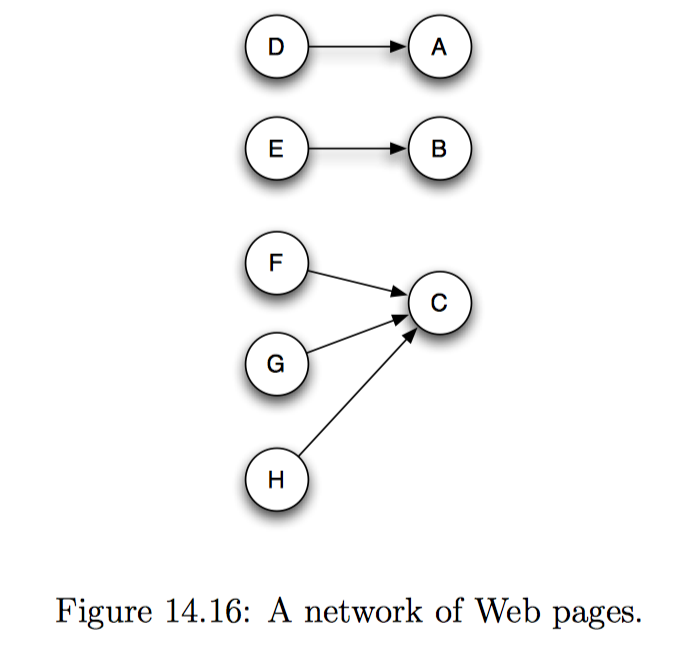
\includegraphics[scale=0.5]{fig1.png}
\end{center}

\textbf{Solution}:\\

Number of steps k is 2 in this question, so we need update all hub scores and all authority scores twice.\\

\textbf{Before Normalization}:

\begin{center}
  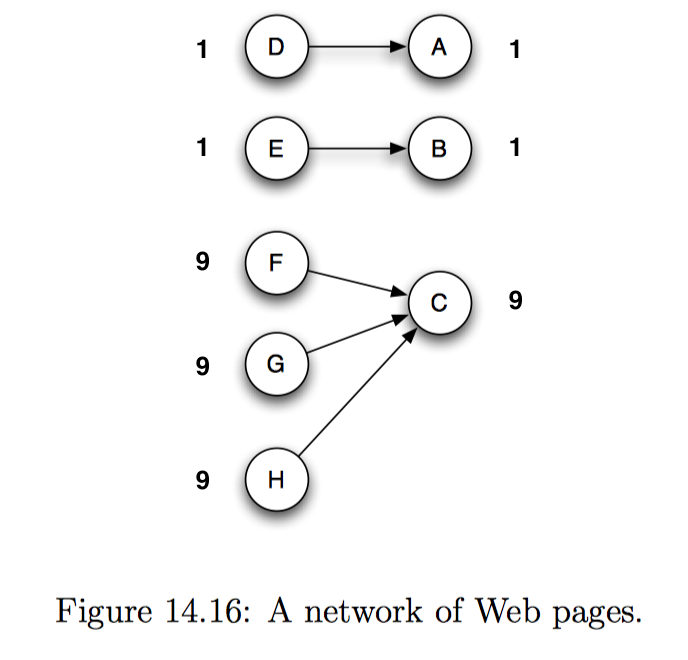
\includegraphics[scale=0.5]{fig1-prev.png}
\end{center}

The steps to reach this result is that, I first initialize hub scores and authority scores to be 1. A single application of the Authority Update Rule followed by a single application the Hub Update Rule produces the results of the original list-finding technique. So in 2 iterations, update \textit{auth(p)} to be the sum of the hub scores of all pages that point to it and update \textit{hub(p)} to be the sum of the authority scores of all pages that it points to.


\textbf{After Normalization}:

\begin{center}
  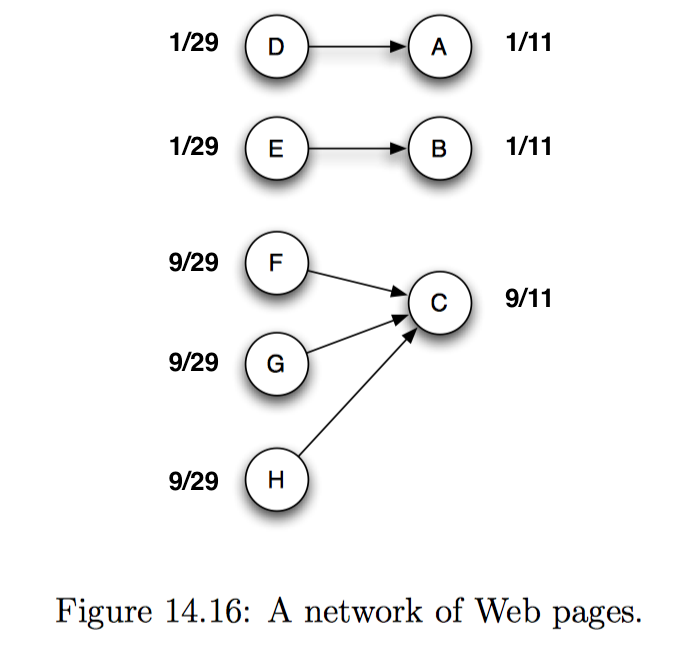
\includegraphics[scale=0.5]{fig1-after.png}
\end{center}

For normalization, we need divide each hub score and each authority score by the sum of all the hub scores and authority scores separately.

\subsection{2. (b)}

Due to the symmetry of nodes A and B in part (a), you should have seen that they get the same authority scores. Now let’s look at what happens to the scores when node E, which links to B, decides to link to C as well. This produces the new network of Web pages shown in Figure 14.17.\\
Similarly to part (a), show the normalized hub and authority values that each node gets when you run the 2-step hub-authority computation on the new network in Figure 14.17.

\begin{center}
  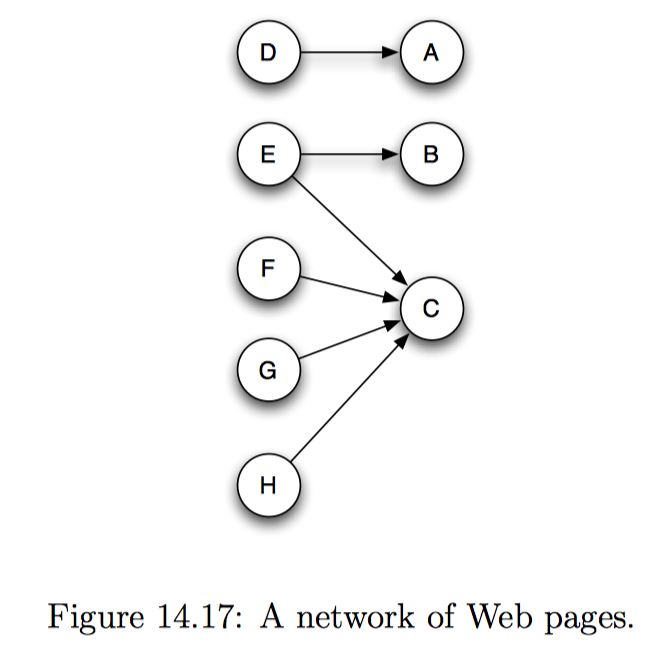
\includegraphics[scale=0.5]{fig2.png}
\end{center}

\textbf{Solution}:

\textbf{After normalization}:

In this case, because node E points to Node C, when we calculate Hub score for Node E, the "input" authority scores come from Node B and Node C. So this breaks the symmetry.

\begin{center}
  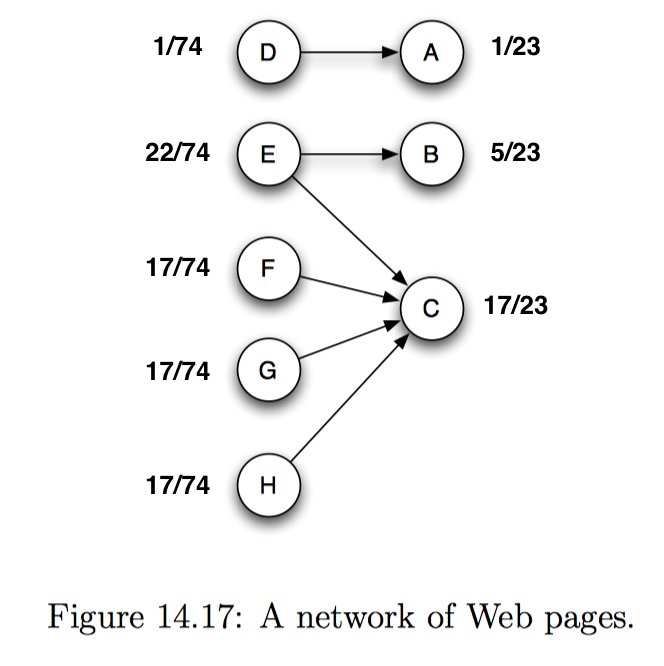
\includegraphics[scale=0.5]{fig2-norm.png}
\end{center}


\subsection{2. (c)}

In (b), which of nodes A or B now has the higher authority score? Give a brief explanation in which you provide some intuition for why the difference in authority scores between A and B in (b) turned out the way it did.

\textbf{Solution}:\\

The input hub score for Node A is from Node D and input hub score for Node B is from Node E. However, Node E also points to Node C, which has lots of input Nodes. After Authority Update Rule and Hub Update Rule, Node B will have a higher authority score.

\newpage

\section{Question 2 (10 points)}

\subsection{3. (a)}

Show the values that you get if you run two rounds of computing hub and authority values on the network of Web pages in Figure 14.18. (That is, the values computed by the k-step hub-authority computation when we choose the number of steps k to be 2.)

Show the values both before and after the final normalization step, in which we divide each authority score by the sum of all authority scores, and divide each hub score by the sum of all hub scores.

\begin{center}
  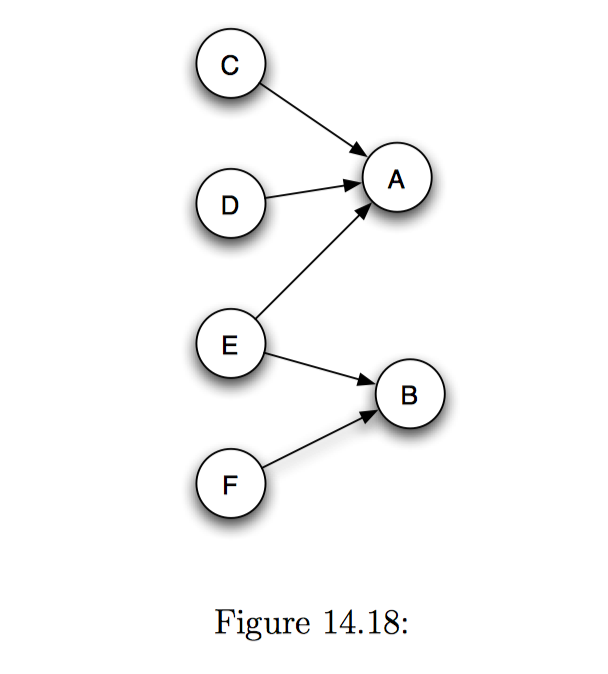
\includegraphics[scale=0.5]{fig3.png}
\end{center}

\textbf{Solution}:

\textbf{Before Normalization}:

\begin{center}
  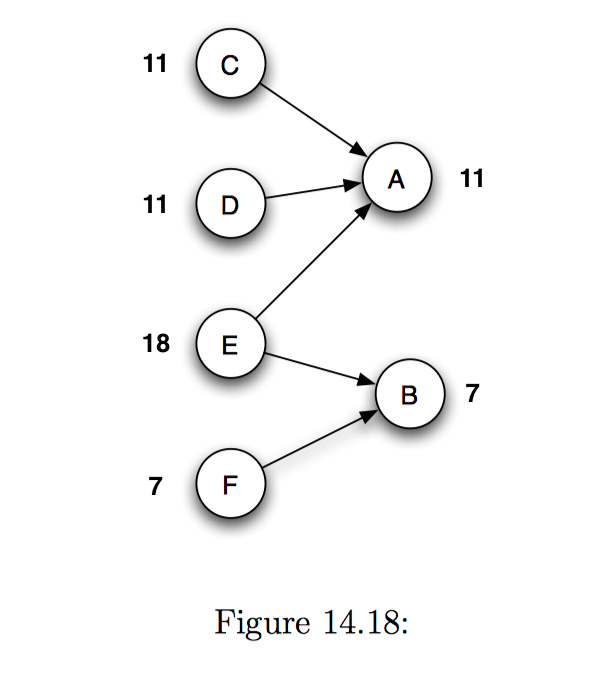
\includegraphics[scale=0.5]{fig3-prev.png}
\end{center}

\textbf{After Normalization}:

\begin{center}
  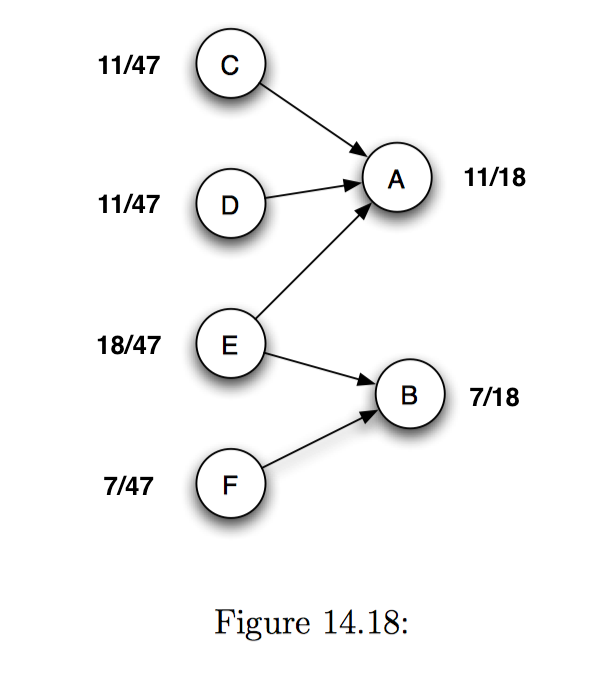
\includegraphics[scale=0.5]{fig3-norm.png}
\end{center}


\subsection{3. (b)}

\textbf{Option 1}:

\begin{center}
  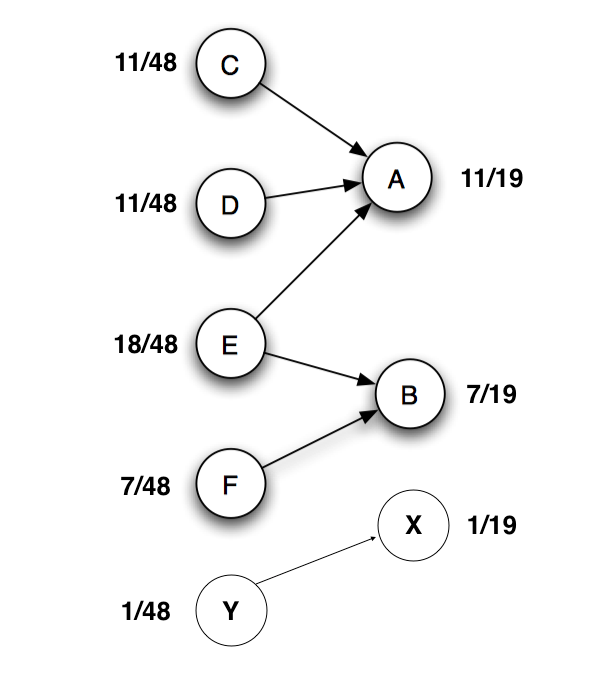
\includegraphics[scale=0.5]{fig4-op1.png}
\end{center}

\textbf{Option 2}:

\begin{center}
  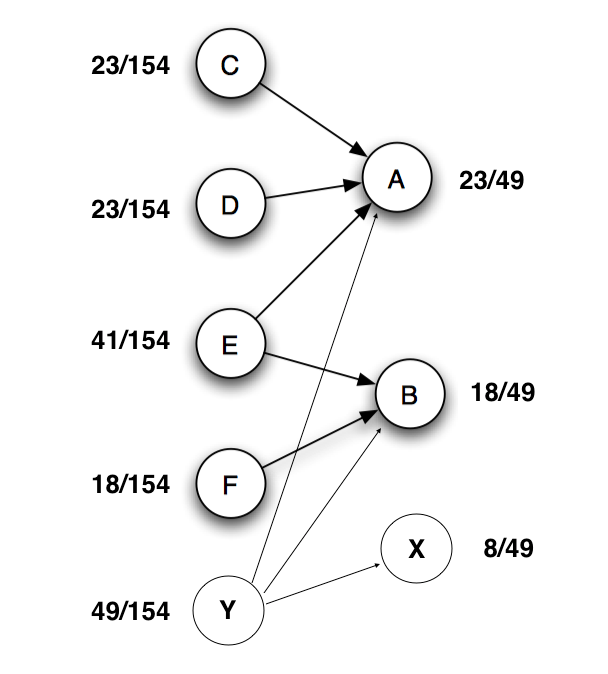
\includegraphics[scale=0.5]{fig4-op2.png}
\end{center}


Option 2 gives higher authority score. Because Node Y points to 3 other Nodes, this make the Updating Hub score for Node Y takes more scores into account. So the authority score of Node X is much higher than Option 1.

\subsection{3. (c)}

\textbf{Solution}:\\

\begin{center}
  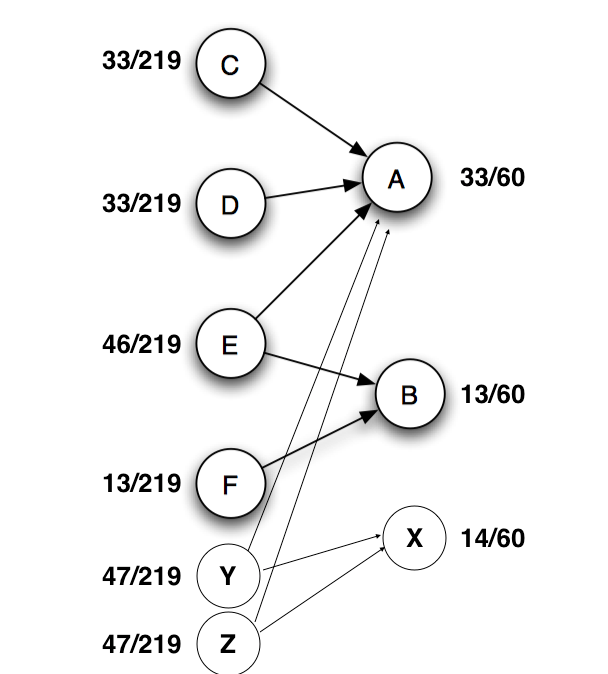
\includegraphics[scale=0.5]{fig4-c.png}
\end{center}


The strategy for placing Node X, Y and Z is that since we would like to place Node X at the second position when we rank the pages, then "incoming" hub scores to Node X is supposed to as high as possible, it will not be higher than Node A, but can be higher than Node B. So Node Y and Z should not connect to Node B. This will keep the "incoming" hub scores of Node B the same but increase them of Node X.


\newpage

\section{Question 4 (2 points)}

\begin{itemize}
\item Review movies with high authority scores.
\item No, the effects in small graphs are more obvious than larger ones.
\end{itemize}


\end{document}